%Preamble:
\documentclass[12pt,onecolumn,letterpaper]{article} %possibilities: book, report, etc
%change the fontsize to 12pt, etc if desired
%Also possible \documentclass[10pt,twocolumn]{article}
%Also possible: \documentclass{CSUthesis} (our template)





%Change margins: Usually taken care of by style file from journal, etc.
\textwidth=6.85in
\oddsidemargin=-0.5in
\textheight=9in
\topmargin=-0.75in



\makeatletter
\newcommand*{\encircled}[1]{\relax\ifmmode\mathpalette\@encircled@math{#1}\else\@encircled{#1}\fi}
\newcommand*{\@encircled@math}[2]{\@encircled{$\m@th#1#2$}}
\newcommand*{\@encircled}[1]{%
  \tikz[baseline,anchor=base]{\node[draw,circle,outer sep=0pt,inner sep=.2ex] {#1};}}
\makeatother
\newcommand{\tens}[1]{%
  \mathbin{\mathop{\otimes}\displaylimits_{#1}}%
}
\usepackage{cancel}
\usepackage{graphicx}
\usepackage{bigints}
\usepackage{tikz}
\usepackage{amsmath}
\usepackage{framed}
\usepackage{amssymb}
\usepackage[inline]{enumitem}
\usepackage{amsmath}
\usepackage{framed}
\usepackage{amsmath}
\usepackage{amssymb}
\usepackage[inline]{enumitem}
\usepackage{amsmath}
\usepackage{framed}
\usepackage{amsmath}
\usepackage{breqn}
\usepackage[utf8]{inputenc}
\usepackage{dirtytalk}
\usepackage{booktabs}
\usepackage{multirow}
\usepackage{url,epsfig,graphics,float}
\usepackage{color}
\usepackage{subcaption}
\renewcommand{\baselinestretch}{1.5}
\usepackage{tikz}
\usepackage{blindtext}
\begin{document}
\begin{titlepage}
\begin{center}

% Upper part of the page. The '~' is needed because \\
% only works if a paragraph has started.

\textsc{\LARGE MTH 593 Exit Project  }\\[0.5cm]
\textsc{\Large Fall 2018}\\[4cm]

\includegraphics[width=0.35\linewidth]{temp.JPG}\\[2cm]



% Title
%\HRule \\[0.4cm]
%{ \huge \bfseries Lager brewing techniques \\[0.4cm] }

%\HRule \\[1.5cm]
\textsc{\Large Topic:  Clifford Algebra-Study of Linkages}\\[2cm]

% Author and supervisor
\begin{minipage}{0.4\textwidth}
\begin{flushleft} \large
\emph{Students:}\\

Shola \textsc{Otitoju}\\

\end{flushleft}
\end{minipage}
\begin{minipage}{0.4\textwidth}
\begin{flushright} \large
\emph{Instructors:} \\

Dr. Jonathan \textsc{Scott}
 
  
\end{flushright}
\end{minipage}

\vfill

% Bottom of the page
{\large August 2018}

\end{center}
\end{titlepage}
%%%%%%%%%%%%%%%%%%%%%%%%%%%%%%%%%%%%%%%%%%%%%%%%%
\tableofcontents
\listoffigures
%\listoftables

\section{Introduction}
Motion of rigid bodies finds rich application in mechanisms and robots used for automation in industries. They are used to optimally plan the motion path of these kind of mechanisms, such that several of these mechanisms working together in say a production process always avoid colliding with each other and also, carry out their task in an effective and efficient manner. \\
Each of these mechanism or robot is itself a multi-body system that is made up of several linkages connected at joints(prismatic or revolute type), with each linkage having relative motion with the one adjacent to it.\\ To arrive at a desired end effector pose (The position of the $n^{th}$ linkage which interacts with the environment), the pose and motion of the other $n-1$ linkages have to be planed as well. Transformations that relates end points (vectors) of each linkage from their local frame to the base (or ground) frame are carried out. This allows us to convert the coordinates of a point from each frame to the base frame, which gives expressions that describes the position and orientation of the whole mechanism linkage by linkage.\\
Typically, they are homogeneous transformation matrices ($SE(3)$, Special Euclidean
Group) that combines rotation of each joints in different planes and possibly some translation. For example, if we have a linkage $l_i$ with end point represented by the vector $\vec{l}^0_i=a_0e_1+b_0e_2+c_0e_3$, a rotation of  this linkage by $\theta$, $\alpha$ and $\gamma$ about the $x$, $y$ and $z$-axis will give its new position $\vec{l}^1_i=a_1e_1+b_1e_2+c_1e_3$ as.
\begin{equation}
  \large  \left [
\begin{array}{l}
a_1  \\
b_1  \\
c_1
\end{array} \right]=\large{R^1_0}   \left [
\begin{array}{l}
a_0  \\
b_0  \\
c_0
\end{array} \right]
\end{equation}
where
\begin{align*}
R^1_0=R^1_{Z,\gamma}R^1_{y,\alpha}R^1_{x,\theta}=
\left [
\begin{array}{llr}
\cos\gamma & -\sin\gamma & 0 \\
\sin\gamma & \cos\gamma  & 0 \\
0 & 0 & 1
\end{array} \right]
\left [
\begin{array}{llr}
\cos\alpha & 0 & \sin\alpha \\
0 & 1 & 0 \\
-\sin\alpha & 0 & \cos\alpha
\end{array} \right]
\left [
\begin{array}{llr}
1 & 0 & 0 \\
0 & \cos\theta & -\sin\theta \\
0 & \sin\theta & \cos\theta
\end{array} \right]
\end{align*}
which gives:
\begin{align}
R^1_0=
\left [
\begin{array}{llr}
\cos\alpha \cos\gamma & \cos\gamma\sin\alpha\sin\theta-\cos\theta\sin\gamma & \sin\gamma\sin\theta+\cos\gamma\cos\theta\sin\alpha \\
\cos\alpha\sin\gamma & \cos\gamma\cos\theta+\sin\alpha\sin\gamma\sin\theta  & \cos\theta\sin\alpha\sin\gamma-\cos\gamma\sin\theta \\
-\sin\alpha & \cos\alpha\sin\theta & \cos\alpha\cos\theta
\end{array} \right]
\label{rotate}
\end{align}
Equation~\ref{rotate} is found by composing the rotations about $x$, $y$ and $z$-axis.\\
We see that for a mechanism with several linkages and joint, the degree of freedom is higher and we can arrive at really large matrices. This motivates the use of Clifford algebra. It allow us to represent each linkages as vectors transformations can be performed algebraically without the need to represent them in large complicated matrices.\\ We therefore explore the use of Clifford algebra for rotation of rigid linkages in this project. The remaining sections will be arranged as follows; In section~\ref{Cliffordd} a brief overview of Clifford algebra and their properties will be presented. This is followed by an overview of Clifford groups, particularly the Spinors and Pinors in section~\ref{Groupss}. Section~\ref{review} give 
a review of some application of geometric algebra and lastly, in section~\ref{apply}, we will apply Clifford algebra in representing the pose and motion of a rigid linkage mechanism.
\section{Clifford algebra}\label{Cliffordd}
 Clifford Algebra is described as a unifying language for mathematics and physics, it is said to be the most extraordinary synergistic confluence of a diverse range of specialized mathematical fields, each with its own methods and formulation, which has found rich applications in areas such as quantum physics, robotics, signal processing, ray tracing, virtual reality, computer vision, vector field processing, tracking, geographic information systems and neural computing~\cite{lundholm2009clifford,lehar2014visual,baker2012matrix}.\\
\indent Clifford algebra is an algebra generated by vector spaces defined over both the real and complex field. They form a generalization for the real numbers, vectors, complex numbers, quaternions and other hypercomplex number systems.\\
\indent Clifford algebra is generally represented as $Cl_n(p,q,r)\in\mathbb{R}^{n^2}$ and can be defined as all element and algebra of the higher order vector space with dimension $2^n$ defined over $T(V)/I(Q)$, where $T(V)$ is the tensor algebra over the vector space $\vec{V}\in\mathbb{R}^{n}$ and $I$ is a particular ideal of the tensor algebra.\\
The vector space $\vec{V}\in\mathbb{R}^{n}$ having bases $e_i$ such that $n=p+q+r$ and:  %where $n=p+q+r$ and $p$, $q$, and $r$ are the number of bases which squares to $1$, the number of bases which squares to $-1$ and the number of bases which squares to $0$. That is:
 \begin{equation}
  (e_i)^2= \begin{cases} 
      1\ \hspace{0.5cm}{\mbox{ for }} 1\le i \le p \\
      -1\ \hspace{0.4cm}{\mbox{ for }} p+1\le i \le p+q \\
      0\ \hspace{0.6cm}{\mbox{ for }} p+q+1\le i \le p+q+r
   \end{cases}\label{velocitydependence} 
\end{equation}
Since we explore the representation of the dynamics and transformation of rigid bodies using Clifford algebra, definition of bases that satisfies the axioms and postulates of Euclidean geometry are made. By this definition, a special class of Clifford algebra; The Geometric algebra results ($Cl_n(p,0,r)$ written as $Cl_n(p,r)$ for short).
\subsection{Geometric algebra}
Geometric algebra proposes an alternative vectorial framework constructed over the Euclidean space where lines, areas, volumes and hyper-volumes (dimensions $n>3$) are recognized as structures with magnitude and orientation (vectors in a way) and also allowing additions and products, such as ($line+line$, $line\times line$), ($line+area$, $line\times area$), ($area+area$, $area\times area$), ($line + volume$, $line\times volume$), ($area + volume$, $area\times volume$), ($volume + volume$, $volume\times volume$), etc. These oriented lines, oriented areas and  oriented volumes are represented by vectors, bivectors and trivectors respectively~\cite{vince2009geometric}. \\
For our choice of definition of the basis vectors over these euclidean space, these algebra are defined over a universal property.
\subsection{Universal properties of Clifford algebras}
Given that $A$ is an $\mathbb {R}$-algebra such that $f:\mathbb {R}^n\rightarrow A$ is an $\mathbb {R}$-linear transformation for which
$$f(x)^2=|x|^21 \hspace{0.8cm} (x\in \mathbb {R}^n)$$
Then there is a unique homomorphism of $\mathbb {R}$-algebras $F:Cl_n\rightarrow A$ for which $F\circ j_n$. That is, for all $x\in \mathbb {R}^n$, $F(j_n(x))=f(x)$ (Fig.~\ref{forceshape}).
\begin{figure}[h]
\centering 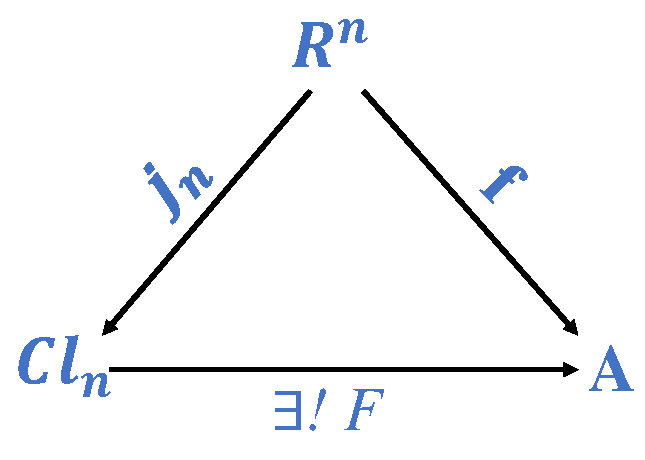
\includegraphics[width=0.3\linewidth]{PICMSTT}
\caption{Commutative diagram} \label{forceshape}
\end{figure}
\begin{equation}
    F\circ j_n(x)=f(x)
\end{equation}
Where $j_n$ is another $\mathbb {R}$-linear transformation defined by:
\begin{equation}
    j_n:\mathbb {R}^n\rightarrow Cl_n; \hspace{.5cm} j_n\left(\sum_{r=1}^{n}x_re_r\right) = \sum_{r=1}^{n}x_re_r\label{jtransform}
\end{equation}
for which
$$j_n\left(\sum_{r=1}^{n}x_re_r\right)^2 = \sum_{r=1}^{n}x_r^2=\left|\sum_{r=1}^{n}x_re_r\right|^2$$

\subsection{Geometric product}
\indent Core to Geometric algebra is its multiplication operation, the geometric product. It unites the Grassmann and Hamilton algebras into a single structure.  Geometric product results in a linear combination of basis elements on a multivector space. Given two arbitrary vectors $\vec{u},\vec{v}\in\mathbb{R}^n$ their geometric product is defined as the sum of their inner product (dot product) and their exterior product (wedge product). That is: 
%% Adding the dual of the Grassmann exterior product (the "meet") allows the use of the Grassmann–Cayley algebra, and a conformal version of the latter together with a conformal Clifford algebra yields a conformal geometric algebra (CGA) providing a framework for classical geometries.[1] In practice, these and several derived operations allow a correspondence of elements, subspaces and operations of the algebra with geometric interpretations.

\begin{equation}\vec{u}\vec{v}=\vec{u} \boldsymbol{\cdot} \vec{v}+\vec{u}\wedge\vec{v}\label{ga1}
\end{equation}
Where $\vec{u} \boldsymbol{\cdot} \vec{v}$ and $\vec{u}\wedge\vec{v}$ is the inner product and the exterior product of the vectors respectively.\\
To discuss the properties of the geometric product, we shall firstly, do a preliminary review of the inner product and the exterior product.
\subsubsection{Preliminaries}
\begin{enumerate}
    \item \textbf{Dot Product:}\\
    The dot product, also known as scalar product is a bilinear mapping from the vector space to a scalar. It is defined as:
    $$(\boldsymbol{\cdot}):\mathbb{R}^{2n} \rightarrow \mathbb{R}$$
     It is evaluated by taking the product of both vectors with the following rules.
      \begin{equation}
      e_i\boldsymbol{\cdot}e_j= \begin{cases} 
      1\ {\mbox{ for }} i= j \\
      0\ {\mbox{ for }} i \neq j
   \end{cases}\label{dott}
   \end{equation}
   For example, given the following vectors:
    $$\vec{u} =a_1\vec{e}_1+a_2\vec{e}2+a_3\vec{e}_3$$
    $$\vec{v}=b_1\vec{e}_1+b_2\vec{e}_2+b_3\vec{e}_3$$
     The inner product is $\vec{u} \boldsymbol{\cdot} \vec{v}$ and it can be directly computed using the properties in eq.~\ref{dott}, as follows:
   
 $$\vec{u} \boldsymbol{\cdot} \vec{v}=(a_1\vec{e}_1+a_2\vec{e}2+a_3\vec{e}_3) \boldsymbol{\cdot} (b_1\vec{e}_1+b_2\vec{e}_2+b_3\vec{e}_3)=a_1b_1+a_2b_2+a_3b_3$$
   The inner product is also equivalent to the product of the magnitude of the vectors and the cosine of the angle between them.
   That is:
   \begin{equation}\vec{A} \boldsymbol{\cdot} \vec{B}=\|A\|\|B\|\cos\theta\end{equation}
   Where $\theta$ is the angle between the vectors.\\

\item \textbf{Exterior product:}\\
The exterior product also called the wedge product is defined as a higher order vector space $\vec{V} \wedge \vec{V}$. Given the vector space $\vec{V}$, $\vec{V} \wedge \vec{V}$ is defined as the subspace in the tensor product $\vec{V}$ $\tens{}$ $\vec{V}$ consisting of all antisymmetric tensors. That is,
$$\vec{v_1} \wedge \vec{v_2}=\vec{v}_1 \tens{} \vec{v}_2 -\vec{v}_2 \tens{}\vec{v}_1,$$
for all $$\vec{v}_1,\vec{v_2}\in \vec{V}$$
This definition can be extended to more than two vectors. If we consider $k$ vectors, then we have that the $k$ exterior product is the subspace of all totally antisymmetric tensors within the tensor product $\vec{V}\tens{}\dots\tens{}\vec{V} $. written as:
$$\vec{v}_1 \wedge \vec{v}_2 \wedge \dots \wedge \vec{v}_k$$ for $$\vec{v}_j\in \vec{V}$$
For short, we write:
$$\vec{v}_1 \wedge \vec{v}_2 \wedge \dots \wedge \vec{v}_k=\wedge^k\vec{V}$$
This product can be computed directly by following certain rules (properties). In order to derive these properties, we shall consider the case of two vectors in two dimensions (fig.~\ref{doublexx}-A). The exterior product of these vectors $\vec{u}\wedge\vec{v}$ is geometrically interpreted as the area of the parallelogram formed by the vectors with the orientation $\vec{uv}$, in this case, clockwise.\\
If we evaluate the exterior product $\vec{v}\wedge\vec{u}$ instead, it will have the same magnitude (the same area) as $\vec{u}\wedge\vec{v}$ but with an opposite orientation. Therefore, exterior products are anticommutative which agrees with its definition.\\That is,
$$\vec{v}\wedge\vec{u}=-\vec{u}\wedge\vec{v}$$
Similarly, the exterior product of three vectors, $\vec{u}\wedge\vec{v}\wedge\vec{w}$ (fig.~\ref{doublexx}-B) is interpreted as the volume of the cuboid formed by the three vectors with an orientation in the order in which this product is evaluated.\\
\begin{figure}[h]
\centering 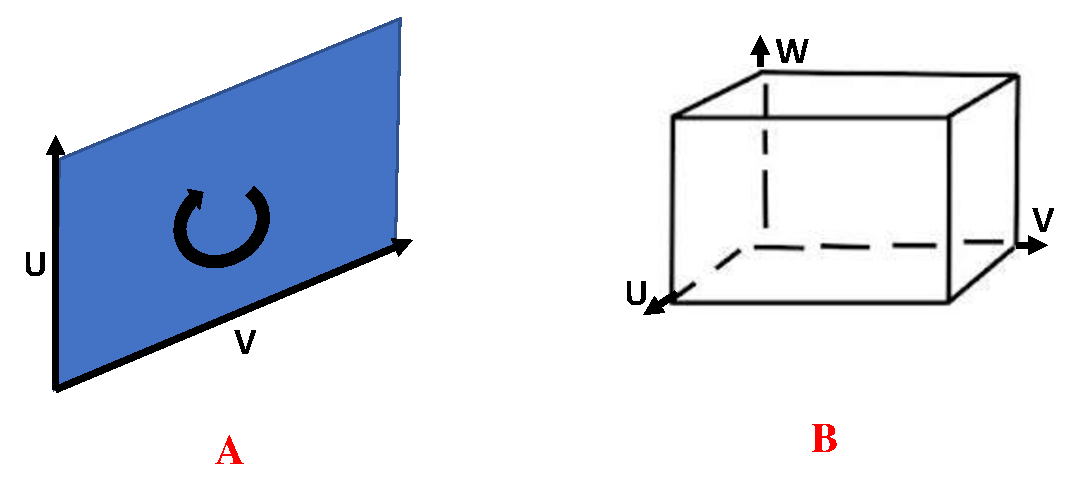
\includegraphics[width=0.6\linewidth]{WEDGE1}\caption{Geometric interpretation of wedge product} \label{doublexx}
\end{figure}
If the exterior product of a vector on itself is taken, say $\vec{u}\wedge\vec{u}$, this result to zero. This is obvious, as we can see that the area enclose by a vector and itself is zero, therefore, such a product gives zero.\\
In summary, the exterior product of vectors is the product of these vectors such that;
\begin{equation*}
  \vec{v}_i\wedge\vec{v}_j= \begin{cases} 
      -\vec{v}_j\wedge\vec{v}_i\ {\mbox{ for }} i\neq j \\
      0\ \hspace{1.2cm}{\mbox{ for }} i = j
   \end{cases}\label{wedgee} 
\end{equation*}
This product is also associative and distributive.\\
As an example, given two vectors defined as:
$$\vec{u}=a_1\vec{e}_1+a_2\vec{e}_2$$
$$\vec{v}=b_1\vec{e}_1+b_2\vec{e}_2$$
then 
$$\vec{u}\wedge\vec{v}=(a_1\vec{e}_1+a_2\vec{e}_2)\wedge(b_1\vec{e}_1+b_2\vec{e}_2)$$
$$=a_1b_1(\vec{e}_1\wedge\vec{e}_1)+a_2b_2(\vec{e}_2\wedge\vec{e}_2)+a_1b_2(\vec{e}_1\wedge\vec{e}_2)+a_2b_1(\vec{e}_2\wedge\vec{e}_1)$$
but $(\vec{e}_1\wedge\vec{e}_1)=(\vec{e}_2\wedge\vec{e}_2)=0$ and  $(\vec{e}_2\wedge\vec{e}_1)=-(\vec{e}_1\wedge\vec{e}_2)$.\\
therefore,
$$\vec{u}\wedge\vec{v}=(a_1b_2-a_2b_1)(\vec{e}_1\wedge\vec{e}_2)$$
The result is neither a scalar or a vector, it is a bivector (a multivector in the plane).
\end{enumerate}
Now that we have done a brief review of both the inner product and the exterior product, we shall now discuss the properties of the geometric product.
\subsubsection{Properties of the Geometric Product operation}
Recall the definition of the geometric product given by eq.~\ref{ga1}, if we consider two arbitrary vectors $\vec{a}$ and $\vec{b}$.\\
Given that $\vec{u}=a_1\vec{e}_1+a_2\vec{e}_2$ and $\vec{v}=b_1\vec{e}_1+b_2\vec{e}_2$, the the geometric product simplifies to:
$$\vec{u}\vec{v}=(a_1b_1+a_2b_2)+(a_1b_2-a_2b_1)(\vec{e}_1\wedge\vec{e}_2)$$
Similarly, if both vectors are in $\mathbb{R}^3$, i.e,  $\vec{u}=a_1\vec{e}_1+a_2\vec{e}_2+a_3\vec{e}_3$ and $\vec{v}=b_1\vec{e}_1+b_2\vec{e}_2+b_3\vec{e}_3$, the geometric product reduces to:
$$\vec{u}\vec{v}=(a_1b_1+a_2b_2+a_3b_3)+(a_1b_2-a_2b_1)(\vec{e}_1\wedge\vec{e}_2)+(a_1b_3-a_3b_1)(\vec{e}_1\wedge\vec{e}_3)+(a_2b_3-a_3b_2)(\vec{e}_2\wedge\vec{e}_3)$$
In both cases, we see that the geometric product resulted to the sum of a scalar and bivectors. It will be shown in a later section that the geometric product of two or more vectors will always yield the sum of a scalar and multivectors, and the order of the multivector is dependent on the numbers of vectors been multiplied and the number of basis element in the vector space.\\
We shall also show that the result of a geometric product is isomorphic to the complex numbers.\\

\begin{itemize}
    \item \textbf{Case I: $\vec{a}$ and $\vec{b}$ are parallel to each other}
    If $\vec{b}$ is parallel to $\vec{a}$, then we can express $\vec{b}$ as a scalar multiple of $\vec{a}$. i.e,
    $$\vec{b}=k\vec{a}$$ where $K$ is a scalar.
    The geometric product of these vectors is thus:
    $$\vec{a}\vec{b}=\vec{a} \boldsymbol{\cdot} \vec{b}+\vec{a}\wedge\vec{b}$$
    $$=\vec{a} \boldsymbol{\cdot} (k\vec{a})+\vec{a}\wedge (k\vec{a})$$
    $$=k(\vec{a} \boldsymbol{\cdot} \vec{a}+\vec{a}\wedge \vec{a})$$
    but $\vec{a}\wedge \vec{a}=0$ (area enclosed is zero).
    therefore, the geometric product reduces to:
    $$\vec{a}\vec{b}=k(\vec{a} \boldsymbol{\cdot} \vec{a})$$
    $$\vec{a}\vec{b}=k\|a\|^2$$
    \item \textbf{Case II: $\vec{a}$ and $\vec{b}$ are orthogonal to each other}
    Similarly, we have the geometric product of these vectors as;
    $$\vec{a}\vec{b}=\vec{a} \boldsymbol{\cdot} \vec{b}+\vec{a}\wedge\vec{b}$$
    recall that $\vec{a} \boldsymbol{\cdot} \vec{b}=\|a\|\|b\|\cos\theta$
where $\theta=\frac{\pi}{2}$.\\
Therefore:
$$\vec{a} \boldsymbol{\cdot} \vec{b}=0$$\\
Thus the geometric product reduces to:
$$\vec{a}\vec{b}=\vec{a}\wedge\vec{b}$$
\end{itemize}
In summary, we have that,
\begin{equation}
  \vec{a}\vec{b}= \begin{cases} 
      k\|a\|^2 \hspace{.5cm}{\mbox{ for $\vec{b}=k\vec{a}$  \hspace{.3cm}($\vec{b}\parallel \vec{a}$) }} \\
      \vec{a}\wedge\vec{b}\ \hspace{.5cm}{\mbox{ for $\vec{b}\perp \vec{a}$ }} i = j
   \end{cases}\label{geoprod} 
\end{equation}
This property can be extended to the orthonormal basis vectors of the euclidean space:
\begin{equation}
      \vec{e}_i\vec{e}_j= \begin{cases} 
      1\ \hspace{.7cm}{\mbox{ for }} i= j \\
      \vec{e}_i\wedge\vec{e}_j\ {\mbox{ for }} i \neq j
   \end{cases}
   \end{equation}
   \begin{itemize}
       \item \textbf{Square of a unit bivector}
         \begin{eqnarray*}
    (\vec{e}_i\vec{e}_j)^2&=&\vec{e}_i\vec{e}_j\vec{e}_i\vec{e}_j\\
     &=&-\vec{e}_i\vec{e}_i\vec{e}_j\vec{e}_j\\
   &=& -\vec{e}_j\vec{e}_j\\
    &=& -1
\end{eqnarray*}
Therefore, the square of unit bivectors is:
$$(\vec{e}_i\vec{e}_j)^2=-1$$
   \end{itemize}
We see that unit bivectors square to $-1$ just like the imaginary unit $i$. The geometric product which results into the sum of a scalar and bivectors therefore, are equivalent (isomorphic) to the complex numbers. That is:
\begin{equation}
    \vec{a}\vec{b}=\vec{a} \boldsymbol{\cdot} \vec{b}+\vec{a}\wedge\vec{b}\cong x+iy\label{uform}
\end{equation}
where in this case, $\vec{a},\vec{b}\in\mathbb{R}^{2}$. Also,  $x=\vec{a} \boldsymbol{\cdot} \vec{b}$ and $y=||\vec{a}\wedge\vec{b}||$

\subsubsection{Other properties of the Geometric Product}
\begin{enumerate}
    \item \textbf{Commutative property:}\\
    Consider the geometric product of two vectors $\vec{a}$ and $\vec{b}$.
   \begin{eqnarray*}
    \vec{a}\vec{b}&=&\vec{a}\boldsymbol{\cdot} \vec{b}+\vec{a}\wedge\vec{b}\\
     &=&\vec{b} \boldsymbol{\cdot} \vec{a}-\vec{b}\wedge\vec{a}\\
   &\neq& \vec{b}\vec{a}
\end{eqnarray*}
We can see that in general, the geometric product is neither commutative nor anti-commutative. \\In special cases, If the vectors are parallel, we have that:
 \begin{eqnarray*}
    \vec{a}\vec{b}&=&\vec{a}\boldsymbol{\cdot} \vec{b}\\
     &=&\vec{b} \boldsymbol{\cdot} \vec{a}\\
   &=& \vec{b}\vec{a}
\end{eqnarray*}
 The geometric product will be commutative.\\
   And if they are perpendicular,
    \begin{eqnarray*}
    \vec{a}\vec{b}&=&\vec{a}\wedge\vec{b}\\
     &=&-\vec{b}\wedge\vec{a}\\
   &=& -\vec{b}\vec{a}
\end{eqnarray*}
the geometric product will be anti-commutative.
  \item \textbf{Associative and Distributive property:}\\ 
  From the axioms of the euclidean space, it is trivial that the geometric product is both associative and distributive over addition. That is:
  $$(\vec{u}\vec{v})\vec{w}=\vec{u}(\vec{v}\vec{w})$$
  $$\vec{u}(\vec{v}+\vec{w})=\vec{u}\vec{v}+\vec{u}\vec{w}$$
\end{enumerate}
\subsection{Basis of Geometric algebra}
As have been discussed, Geometric algebra gives a framework constructed over the euclidean space where geometric products of vectors of products hold, giving rise to a higher vector space with possibly scalars, vectors and multivectors as elements. In all, the basis of this higher dimension vector field is therefore the  set of all possible products of $n$ orthogonal basis vectors written in increasing order of indices including $1$ which represent the inner product. \\
Therfore the basis is given by:
\begin{equation}
    \{1,e_{1},e_{2},e_{3},e_{1}e_{2},e_{1}e_{3},e_{2}e_{3},e_{1}e_{2}e_{3}\}
\end{equation}
This basis vectors span the whole geometric algebra space.
\subsection{Generalized Permutation Matrix representation}
In certain applications, it is necessary to represent geometric algebras in matrix form. These representation are referred to as the Genetalized Permutaion Matrix representation. The rationale for finding matrix representations is that efficient algorithms for carrying out numerical computations of systems represented in matrix form exists. Example of such tools used is MATLAB.\\
\indent These matrix representations are orthogonal matrices with determinant of $1$,  whose elements are either zeros, plus one or negative one. And for each row and column, there is exactly one non-zero entry.\\
For example, if we consider a geometric algebra defined over a vector space $\vec{V}\in\mathbb{R}^{2}$, The basis of the geometric algebra is the set:
$$\{1,e_{1},e_{2},e_{1}e_{2},\}$$
An algebra in this space will have the form:
$$Cl_2=a_0+a_1e_{1}+a_2e_{2}+a_{12}e_{1}e_{2}$$
The permutation matrix of this algebra is given by:
$$\rho(Cl_2)=\rho(a_0+a_1e_{1}+a_2e_{2}+a_{12}e_{1}e_{2})=a_0\rho(1)+a_1\rho(e_{1})+a_2\rho(e_{2})+a_{12}\rho(e_{1}e_{2})$$
Where $\rho(1)$, $\rho(e_1)$, $\rho(e_2)$,  and $\rho(e_1e_2)$ are component permutaion matrix of the algebra space. That is:


 \begin{eqnarray*}
    \rho(1)&=&1\{1,e_{1},e_{2},e_{1}e_{2}\}=\left [
\begin{array}{llll}
1 & 0 & 0 & 0 \\
0 & 1 & 0 & 0 \\
0 & 0 & 1 & 0\\
 0 & 0 & 0 & 1
\end{array} \right ]=I_4\\
\rho(e_1)&=&e_1\{1,e_{1},e_{2},e_{1}e_{2}\}=\{e_1,1,e_1e_{2},e_{2}\}=\left[
\begin{array}{llll}
0 & 1 & 0 & 0 \\
1 & 0 & 0 & 0 \\
0 & 0 & 0 & 1\\
 0 & 0 & 1 & 0
\end{array} \right ]
\end{eqnarray*}

\begin{eqnarray*}
\rho(e_2)&=&e_2\{1,e_{1},e_{2},e_{1}e_{2}\}=\{e_2,-e_1e_2,1,-e_{1}\}=\left[
\begin{array}{llll}
0 & 0 & 1 & 0 \\
0 & 0 & 0 & -1 \\
1 & 0 & 0 & 0\\
 0 & -1 & 0 & 0
\end{array} \right ]\\
\rho(e_1e_2)&=&e_1e_2\{1,e_{1},e_{2},e_{1}e_{2}\}=\{e_1e_2,-e_2,e_1,-1\}=\left[
\begin{array}{llll}
0 & 0 & 0 & -1 \\
0 & 0 & 1 & 0 \\
0 & -1 & 0 & 0\\
1 & 0 & 0 & 0
\end{array} \right ]
\end{eqnarray*}
Then, the permutation matrix of the given algebra is:
\begin{eqnarray*}
\rho(Cl_2)=a_0\left [
\begin{array}{llll}
1 & 0 & 0 & 0 \\
0 & 1 & 0 & 0 \\
0 & 0 & 1 & 0\\
 0 & 0 & 0 & 1
\end{array} \right ]+a_1\left[
\begin{array}{llll}
0 & 1 & 0 & 0 \\
1 & 0 & 0 & 0 \\
0 & 0 & 0 & 1\\
 0 & 0 & 1 & 0
\end{array} \right ]+a_2\left[
\begin{array}{llll}
0 & 0 & 1 & 0 \\
0 & 0 & 0 & -1 \\
1 & 0 & 0 & 0\\
 0 & -1 & 0 & 0
\end{array} \right ]+a_{12}\left[
\begin{array}{llll}
0 & 0 & 0 & -1 \\
0 & 0 & 1 & 0 \\
0 & -1 & 0 & 0\\
1 & 0 & 0 & 0
\end{array} \right ]
\end{eqnarray*}
which reduces to:
\begin{equation}
    \rho(a_0+a_1e_{1}+a_2e_{2}+a_{12}e_{1}e_{2})=\left[
\begin{array}{llll}
a_0 & a_1 & a_2 & -a_{12} \\
a_1 & a_0 & a_{12} & -a_2 \\
a_2 & -a_{12} & a_0 & a_1\\
 a_{12} & -a_2 & a_1 & a_0
\end{array} \right ]
\end{equation}
\section{Clifford Groups}\label{Groupss}
Given a finite dimensional vector space $\vec{V}\in \mathbb{R}^n$, the clifford group is the subgroup defined by:
\begin{equation}
    \Gamma_n=\{u\in Cl_n^{\times} : \forall x\in\vec{V}, \alpha(u)xu^{-1}\in\vec{V}\}\le  Cl_n^X\label{cliffordg}
\end{equation}
Where $Cl_n^{\times}$ is the multiplicative group of invertible elements $Cl_n$ and $\alpha$ is a unique canonical automorphism (see definitions).
\subsection{Some selected Propositions and their proofs}
Here, some proposition are discussed. They are necessary to further study the Clifford groups that are of interest to us. Before these propositions are discussed, some underlining definitions and theorems will be made.
\begin{itemize}
   \item  \textbf{\emph{Definition 1:} Continuous Group Action}\label{action}\\
    An action $\mu$ of a group $G$ on a set $X$ is a function $\mu : G\times X\to X$ satisfying the following conditions for all $g,h\in G$ and $x\in X$ and  $\jmath$ being the identity element of $G$:
     \begin{eqnarray*}
     (gh)x&=&g(hx)\hspace{.5cm} i.e, \hspace{.5cm} \mu(gh,x)=\mu(g,\mu(h,x))\\
     \jmath x&=&x
      \end{eqnarray*}
      This group action $\mu$ has two important notation.
      \begin{enumerate}
          \item \textbf{Stabilizer:}\\
          For $x\in X$, the stabilizer of x is
          \begin{equation}
              Stab_G(x)=\{g\in G : gx=x\}\subseteq G \label{stab}
          \end{equation}
          \item \textbf{Orbit:}\\
          For $x\in X$, the orbit of x is
          \begin{equation}
              Orb_G(x)=\{gx\in X : g\in G\}\subseteq X \label{orbit}
          \end{equation}
      \end{enumerate}
\item  \textbf{Theorem 1:}\\
Given that the $G$ act on  the set $X$, then;
\begin{enumerate}[label=\roman*.]
\item For $x\in X$, $Stab_G(x)\le G$, i.e, $Stab_G(x)$ is a subgroup of $G$.
\item For $x,y\in X$, then $y\in Orb_G(x)$ if and only if $Orb_G(y)=Orb_G(x)$.
\item For $x\in X$, there is a bijection
$$\psi : G/Stab_G(x)\to Orb_G(x); \hspace{.5cm} i.e, \hspace{.5cm}\psi(g)=gx$$
also, for all $g,h\in G$,
$$\psi((hg(x)Stab_G(x))=h\psi(g Stab_G(x))$$
\item If $y\in Orb_G(x)$, the for any $t\in G$ satisfying $y=tx$,
$$Stab_G(y)=tStab_G(x)t^{-1}$$
\end{enumerate}
\item  \textbf{\emph{Definition 2:} Conjugation and Ring Anti-homomorphism}\\
Given the Clifford algebra $Cl_n$, the exist a conjugation $\overline{(\hspace{.2cm} )} : Cl_n\to Cl_n$ defined by
$$\overline{e_{i_1}e_{i_2}\dots e_{i_k}}=(-1)^ke_{i_k}e_{i_{k-1}}\dots e_{i_1}$$
whenever $1\le i_1\le i_2\le \dots \le i_k\le n$ satisfying
$$\overline{x+y}=\overline{x}+\overline{y}$$ and 
$$\overline{tx}=t\overline{x}$$
for $x,y\in Cl_n$ and $t\in \mathbb{R}$
For $n>1$, the above conjugation is a Ring Anti-homomorphism in the sense that for all $x,y\in Cl_n$
\begin{equation}
    \overline{xy}=\overline{y}\hspace{.08cm}\overline{x}\label{conjugate}
\end{equation}
\item  \textbf{\emph{Definition 3:} Canonical Automorphism and grading on $Cl_n$}\\
$\alpha$ is a unique canonical automorphsim $\alpha : Cl_n \to Cl_n$ with properties
$$\alpha\circ \alpha=id$$
$$\alpha(i(v))=-i(v)$$
This canonical automorphism $\alpha$ can be used to define a ($+$)-grading and a ($-$)-grading on $Cl_n$ as follows: 
$$Cl_n^{+}=\{u\in Cl_n : \alpha(u)=u\},\hspace{1cm}Cl_n^{-}=\{u\in Cl_n : \alpha(u)=-u\}$$
By this grading, the following holds:
\begin{enumerate}[label=\roman*.]
\item Every element $v \in Cl_n$ can be uniquely decomposed as $v=v^++v^-$ such that $v^+\in Cl_n^{+}$ and $v^-\in Cl_n^{-}$.
\item This decomposition is multiplicative, that is; 
\begin{equation}
       \begin{cases} 
      uv,vu\in Cl_n^{+} \hspace{.7cm}{\mbox{if  }} u,v\in Cl_n^{+} \hspace{.2cm}{\mbox{or  }} u,v \in Cl_n^{-} \\
      uv,vu\in Cl_n^{-} \hspace{.7cm}{\mbox{if  }} u\in Cl_n^{+} \hspace{.2cm}{\mbox{and  }} v \in Cl_n^{-}\label{decompose}
   \end{cases}
   \end{equation}
\end{enumerate}
\item  \textbf{\emph{Definition 4:} $\mathbb{R}$-linear isometry defined over  $\Gamma_n$}\\
For all $u\in \Gamma_n$, there exists an $\mathbb{R}$-linear isometry $\rho_u : \mathbb{R}^n\to\mathbb{R}^n $ such that
$$|\rho_u(x)|=|x|^2$$
for all $x\in \mathbb{R}$.
By expressing $\rho_u$ for any $u\in\Gamma_n$ in terms of the the standard basis, we have that
$$|\rho_u(e_i)|=1, \hspace{.5cm} i=1,2,\dots, n$$
Therefore we have that $\rho_u\in O(n)$ and there is a continuous group homomorphism
\begin{equation}
    \rho :  \Gamma_n\to O(n); \hspace{.5cm}\rho(u)=\rho_u
\end{equation}
and the kernel of $\rho$
\begin{equation}
    ker\hspace{.2cm}\rho =\mathbb{R}^{\times}= \{t1 : t\in \mathbb{R}, t\neq0\}
\end{equation}
\end{itemize}
 \subsubsection{PROPOSITION 1}\label{prop1}
 $\Gamma_n$ is a closed subgroup of $Cl_n^{\times}$\\
 \textbf{\emph{Proof}}\\ 
 By definition of Clifford groups, we can see that:\\
$\alpha(u)$ is a continuous action of the group $Cl_n^{\times}$ acting on $Cl_n$ such that;
$$Cl_n^{\times}\times Cl_n\to Cl_n;\hspace{.5cm}(u,x)=\alpha(u)xu^{-1}$$
 $u\in Cl_n^{\times}$, therefore, there is a linear isomorphism
 $$Cl_n\to Cl_n;\hspace{.5cm}x\mapsto\alpha(u)xu^{-1}$$
 Since $\vec{V}\in \mathbb{R}^n\subseteq Cl_n$, it is a closed $\mathbb{R}$-subspace so by the definition of stabilizers, we have that
 $$\Gamma_n=Stab_{Cl_n^{\times}}\le Cl_n^{\times}$$
 is a closed subgroup of $Cl_n^{\times}$
 \subsubsection{PROPOSITION 2}\label{prop2}
 Given that Clifford group $\Gamma_n$ for $n\ge 1$ is a matrix group, for any $u\in\Gamma_n$, $\alpha(u)$ and $\overline{u}$ are also in $\Gamma_n$.\\
  \textbf{\emph{Proof}}\\
  For $u\in\Gamma_n$,and $x\in \mathbb{R}^n$, the unique canonical automorphism $\alpha(x)=-x=\overline{x}\in \mathbb{R}^n$.\\
  %Combining eqn.~\ref{conjugate} and the fact that for all $u\in Cl_n$, we have that $\alpha(\overline{u})=\overline{\alpha(u)}$ gives:
  From the definition of the Clifford group in Eqn.~\ref{cliffordg}, we have that
  $$\alpha(u)xu^{-1}\in\vec{V}$$
  then the canonical automorphsim map of this is given by,
  $$\alpha(\alpha(u))x\alpha(u^{-1})$$
  using the property $\alpha(\overline{u})=\overline{\alpha(u)}$ and eqn.~\ref{conjugate}, this simplifies to:
  $$\alpha(\alpha(u))\alpha(-x)\alpha(u)^{-1}$$
  which gives:
  $$\alpha\left(\alpha(u)(-x)u^{-1}\right)\in \mathbb{R}^n$$
 Similarly,
   \begin{eqnarray*}
    \alpha(\overline{u})x\overline{u}^{-1}&=&\overline{\alpha(u)}\hspace{.1cm}\overline{(-x)}\hspace{.1cm}\overline{u^{-1}}\\
     &=&\overline{u^{-1}\hspace{.1cm}(-x)\hspace{.1cm}\alpha(u)}\\
   &=& \overline{\alpha(\alpha(u^{-1})\hspace{.1cm}\alpha(-x)\hspace{.1cm}u)}\in \mathbb{R}^n
\end{eqnarray*}
Since $\mathbb{R}^n$ is closed under $\alpha$ and $\overline{(\hspace{.15cm})}$, it implies that $\alpha(u)$ and $\overline{u}$ are both in $\Gamma_n$
 \subsubsection{PROPOSITION 3}\label{prop3}
 Given that for $u\in \Gamma_n$, $u\overline{u}\in \mathbb{R}^{\times}$ and $u\overline{u}=\overline{u}u$, if $v\in\Gamma_n$ also, then
 $$uv\overline{uv}=u\overline{u}v\overline{v}$$
 \textbf{\emph{Proof}}\\ 
 For $u\in\Gamma_n$,$u\overline{u}\in \Gamma_n$ also (by proposition 2)\\
 then
 \begin{eqnarray*}
    \rho_{u\overline{u}}(x)&=&\alpha(u\overline{u})x(u\overline{u})^{-1}\\
     &=&\alpha(u)\alpha(\overline{u})x\overline{u^{-1}}u^{-1}\\
   &=& \alpha(u)\left(\alpha(\overline{u})x\overline{u^{-1}}\right)u^{-1}\\
   &=&\alpha(u)\alpha\left(\overline{u}\hspace{.05cm}\overline{x}\alpha(\overline{u^{-1}})\right)u^{-1}
\end{eqnarray*}
But we have that $\alpha(\overline{x})=x$ and $\alpha(x)=-x=\overline{x}$, hence
 \begin{eqnarray*}
    \rho_{u\overline{u}}(x)&=&\alpha(u)\alpha\left(\overline{\alpha(u^{-1})\hspace{.05cm}xu}\right)u^{-1}\\
     &=&\alpha(u)\alpha\left(-\alpha(u^{-1})\hspace{.05cm}xu\right)u^{-1}\\
   &=& \alpha(u)\alpha\left(\alpha(u^{-1})\hspace{.05cm}xu\right)u^{-1}\\
   &=&\alpha(uu^{-1})x(uu^{-1})=x
\end{eqnarray*}
therefore $\rho_{u\overline{u}}(x)=x$, then we also have that
$$\overline{u}u=u^{-1}u\overline{u}u=u\overline{u}u^{-1}u$$
Therefore, if $v\in\Gamma_n$, then
 $$uv\overline{uv}=uv\overline{v}\hspace{0.05cm}\overline{v}=u\overline{u}v\overline{v}$$
 \subsection{Pinor and Spinor Groups}
The Pinor group $Pin(n)$ is a topological group, bounded as a subset of  the Clifford algebra $Cl_n$. It is the closed, even compact subgroup of $Cl_n^{\times}$.\\
Given the unit sphere defined by
$$S^{n-1}=\{x \in \mathbb{R}^n : |x|=1\}\subseteq Cl_n$$
$Pin(n)$ is defined as
\begin{equation}
    Pin(n)=\{u_1 \dots u_k : k\ge o, u_r \in S^{n-1}\}\subseteq Cl_n^{\times}\label{pinor}
\end{equation}
The $\mathbb{R}$-linear isometry of definition $4$ maps $Pin(n)$ to the orthogonal group $O(n)$. 
$$\rho : Pin(n) \to O(n)$$
That is, given $u\in Pin(n)$, then $\rho_u=\rho(u)\in O(n)$.\\
 The Spinor groups $Spin(n)$ are compact connected  groups of units in the Clifford algebras $Cl_n$~\cite{baker2000introduction,baker2012matrix}.
 The spinor group $Spin(n)$ is a subset of the pinor group $Pin(n)$. It is defined as:
 $$Spin(n)=Pin(n)\cap Cl_n^+\le Pin(n)$$
 $Spin(n)$ can also be defined by restricting $Pin(n)$ by the continuous group homomorphsim $\alpha : Pin(n)\to Pin(n)$. This definition is given by:
 $$Spin(n)=\{u\in Pin(n) : \alpha(u)=u\}\le Pin(n)$$
\subsubsection{PROPOSITION 4}\label{prop4}
The continuous homomorphism $\rho : Pin(n) \to O(n)$ is surjective with kernel  $ker_\rho = \{1, -1\}$\\
\textbf{\emph{Proof}}\\
By definition of the isometry $\rho$, the reflection in the hyperplane orthogonal to $u \in S^{n-1}$ is of the form $\rho_u$.\\
Then, to show that $\rho$ is surjectivity, we have that:\\
for some
$$u_1 \dots u_k \in S^{n-1},\hspace{.5cm} u=u_1 \dots u_k\in ker_\rho; \hspace{.5cm} i.e,\hspace{.5cm} \rho_u=I_n$$
This implies that
$$det\left(\rho_{u_1}\rho_{u_2}\dots\rho_{u_k}\right)=det(\rho_{u_1})det(\rho_{u_2})\dots det(\rho_{u_k})=1$$
Each of the $\rho_r$ is a reflection and therefore has det$\rho_r=-1$. These implies that $k$ must be even which means that $u \in Cl^+$.\\
By this, we have that
$$u^{-1}=u_k \dots u_1=\overline{u}$$
So that for $x\in \mathbb{R}^n$,
\begin{equation}
    x=\rho_u(x)=uxu^{-1}\label{rotor1}
\end{equation}
similarly, $\rho : Spin(n) \to SO(n)$ and also we have that
\begin{equation}
    x^'=\rho_u(x)=uxu^{-1}\label{rotor2}
\end{equation}

where $x,x^'\in \mathbb{R}^n$ and $u,u^{-1}\in Spin(n)$.\\
Geometrically, $Spin(n)$ (Eqn.~\ref{rotor2}) rotates the vector $x$ by reflection to $x^'$. This find extensive use in robotics and manipulation of geometries as we will see in our case study in section~\ref{apply}. 
 \section{Review of some Applications of Geometric Algebra}\label{review}
 This section is dedicated to presenting a review of some applications of Geometric algebra, particularly in physics, computer sciences and mathematics. Some of these applications are as follows:
 
 \subsection{Application to Minkowski spacetime}
 The popular application of Geometric algebra is the Minkowski spacetime, also called the spacetime algebra. It was first developed by David Hestenes in the 1960s who also researched on the field of Geometric Calculus in the 1980s.\\
 The spacetime algebra is defined over a set of basis $\{\gamma_0,\gamma_1,\gamma_2,\gamma_3\}$ with properties
 $$\sigma_i=\gamma_i\gamma_0, \hspace{.5cm} (i=1,2,3)$$
 where the bivectors $\sigma_i$ have properties
$$\sigma_i\boldsymbol{\cdot}\sigma_j=\frac{1}{2}(\sigma_i\sigma_j+\sigma_j\sigma_i)=\delta_{ij}\hspace{1cm} {\mbox{  and }}\hspace{1cm}  \sigma_1\sigma_2\sigma_3=I$$
These properties define a euclidean algebra called the algebra of \emph{relative space}. The usefulness of this algebra can be seen by considering an event $x\in \nu$ that is occurring in the frame $\gamma_{\mu}$, This event will be observed or represented in the $\gamma_0$ frame as:
$$x=x^{\mu}\gamma_{\mu}=x^0\gamma_0+x^i\gamma_i=x^0\gamma_0+x^i\gamma_i\gamma_0\gamma_0=(x^0+x^i\sigma_i)\gamma_0$$
Suppose the same event is observed from another frame $e_\mu$ moving at a velocity of $\nu=\frac{dx}{d\tau}$ relative to $\gamma_0$ such that $\nu^2=1$, the event on this frame will be:
$$x=x\nu\nu=(x\boldsymbol{\cdot}\nu+x\wedge \nu)\nu=(t+\textbf{x})\nu$$
by squaring both sides of this expression, we have that
$$x^2=x\nu\nu x=(x\boldsymbol{\cdot}\nu+x\wedge \nu)(x\boldsymbol{\cdot}\nu+x\wedge \nu)=(t+\textbf{x})(t-\textbf{x})=t^2-\textbf{x}^2$$
This gives the invariant interval for the projection of relative time and space vector called a spacetime split.This finds applications in studies in quantum mechanics.\\
This review of  Minkowski spacetime presented here follows from the account given in the article~\cite{lundholm2006geometric}.
\subsection{Application to Geometric Calculus}
The field of mathematics where differentiation and integration of geometries are done is called geometric calculus. Geometric algebra are widely used in geometric calculus.  They are used to derive very useful theories that encompasses  topics like differential geometry and differential forms.


Given that $F:\mathcal{V}\to G(\mathcal{V})$ is a geometric algebra defined over the arbitrary vector $a\in \mathcal{V}$, the directional derivative of $F$ along an arbitrary vector $b\in \mathcal{V}$ is defined as

\begin{equation*}
    \nabla _{b}F(a)=\lim _{\epsilon \rightarrow 0}{\frac {F(a+\epsilon b)-F(a)}{\epsilon }}
\end{equation*} 
where the limit is taken for scalar $\epsilon$. \\
With $\mathcal{V}$ having basis $\{e_i\}$, we can write $x=x^ie_i$ and $\partial_i :=\partial/\partial x^i:=e_i \triangledown$. The vector derivative is then defined as:

$$\triangledown:=e^ie_i\boldsymbol{\cdot} \triangledown=e^i\partial_i$$
This vector derivative has the properties of a vector and a differential operator. That is
$$\nabla \boldsymbol{\cdot}\langle F\rangle_{r}=\langle\nabla F\rangle_{r-1}\hspace{1cm} {\mbox{  and }}\hspace{1cm}  \nabla \wedge\langle F\rangle_{r}=\langle\nabla F\rangle_{r+1}$$
This properties can be used to evaluate the gradient of a funtion $\phi$ that maps a vector in $\mathcal{V}$ to $\mathbb{R}$ ($\phi:\mathcal{V}\to\mathbb{R}$ )
$$\nabla \phi=e^ie_i\boldsymbol{\cdot}\nabla \phi=e^i\partial_i\phi$$
It can also be used to evaluate the divergence and the curl of a function $f$ that maps a vector to a vector ($f:\mathcal{V}\to\mathcal{V}$ ).
$$\nabla \boldsymbol{\cdot}f=e^i\boldsymbol{\cdot}(\partial_i f)=\partial_if^i\hspace{1cm} {\mbox{  and }}\hspace{1cm}  \nabla \wedge f=e^i\wedge (\partial_i f)=e^i\wedge e^j \partial_i f_j$$
The sum of which gives the gradient of $f$.
$$\nabla f=\nabla \boldsymbol{\cdot}f + \nabla \wedge f$$


Considering $\mathcal{V}\in \mathbb{R}^n$ with basis vectors $\{e_{1},\ldots ,e_{n}\}$, then $e_{1}\wedge e_{2}\wedge \cdots \wedge e_{n}$ is the volume of the n-parallelotope subtended by these basis vectors. The integral of the function $F$ over this volume is defined as:
$$ \int _{V}F(x)\,d^{k}X=\int _{V}F(x)\left(e_{i_{1}}\wedge e_{i_{2}}\wedge \cdots \wedge e_{i_{k}}\right)dx^{i_{1}}dx^{i_{2}}\cdots dx^{i_{k}}$$
This integral can be simplified into thr sum of simplices by triangulation of the space. Given that $\{x_{i}\}$ is the coordinates of the vertices of each triangulation, an average measure $\Delta U_{i}(x)$ of the number of triangulation sharing the vertice is assigned. Then the integral of $F$ with respect to $U(x)$ over this volume is obtained as the limit of finer partitioning of the volume into smaller triangulations, this gives:
$$\int _{V}F\,dU=\lim _{n\rightarrow \infty }\sum _{i=1}^{n}F(x_{i})\,\Delta U_{i}(x)$$
These types of geometric derivatives and integrals have great applications such as in derivation of  generalized expressions for Stokes' theorem.\\
Given a multivector-valued function $\mathsf {L}(A;x)$  of the r-grade input $A$ and general linear position $x$, the fundamental theorem of geometric calculus relating  the integral of a derivative over the volume $V$ to the integral over its boundary is given by:
$$\int _{V}{\dot {\mathsf {L}}}\left({\dot {\nabla }}dX;x\right)=\oint _{\partial V}{\mathsf {L}}(dS;x)$$
This review of geometric calculus presented here follows from the book~\cite{hestenes2012clifford}.

\section{Application to motion of a Rigid body}\label{apply}
We recall from Eqn~\ref{rotor2} that the reflection of a vector $x$ is given by
$$ x^'=\rho_u(x)=uxu^{-1}$$
where  $u,u^{-1}\in Spin(n)$,  $u=u_1 \dots u_k$.\\
Particularly, when $k$ is odd, we have net reflection of $x$ and when $k$ is even, the result is a rotation of $x$ by some angle $\theta$, that is, the double reflection of a vector in a given plane rsults in the rotation of the vector.\\
Since our application is in the euclidean space, we will only consider the first two cases mentioned $k=1$ and $k=2$. Where $u_k$ are in the plane in which the vector $x$ is reflected or rotated but $x$ do not have to be in that plane.\\
Let us consider an example to show how the double reflection vectors can be used to rotate a linkage about a given plane.\\
\begin{figure}[h]
\centering 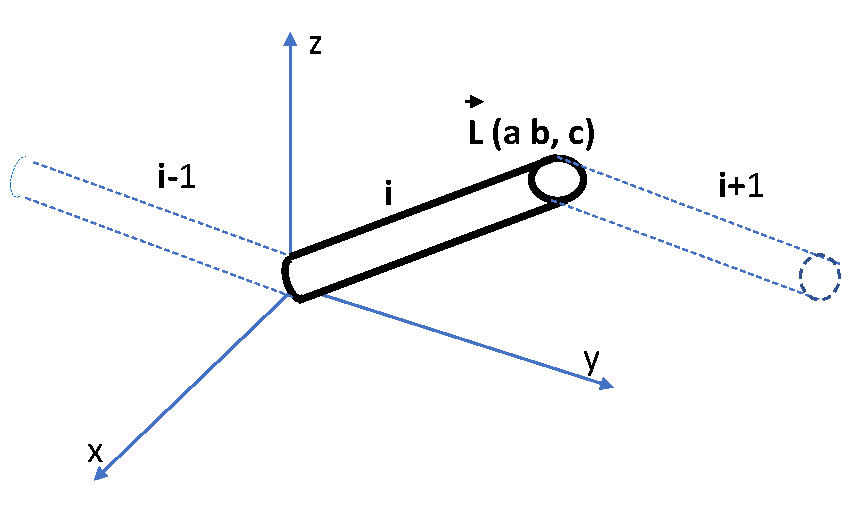
\includegraphics[width=0.6\linewidth]{linkage}\caption{The $i^{th}$ linkage in a mechanism} \label{linkage}
\end{figure}
Figure~\ref{linkage} represents the $i^{th}$ linkage in a mechanism that has several, linkages connected to each other. We will use Eqn~\ref{rotor2} to carry out some rotations of the linkage about it's local frame.\\
First, Let us rotate this linkage by say $\frac{\pi}{4}$ in the $y-z$ plane. This is the same as rotating the linkage by $\frac{\pi}{4}$ about the $x$-axis. For the purpose of comparison, we will also use the rotation matrix from\
Rotating $\vec{L}=\langle a,b,c\rangle$ by $\frac{\pi}{4}$ about the $x$-axis is given by:
\begin{equation*}
\vec{L}_{x=\frac{\pi}{4}}=\large{R^1_x}\vec{L}=  \left [
\begin{array}{llr}
1 & 0 & 0 \\
0 & \cos\frac{\pi}{4} & -\sin\frac{\pi}{4} \\
0 & \sin\frac{\pi}{4} & \cos\frac{\pi}{4}
\end{array} \right] \left [
\begin{array}{l}
a  \\
b  \\
c
\end{array} \right]
\end{equation*}
which simplifies to give:
$$\vec{L}_{x,\frac{\pi}{4}}=\left\langle a, \frac{\sqrt{2}}{2}(b-c), \frac{\sqrt{2}}{2}(b+c)\right\rangle$$
Using the reflection for this same linkage. We have $u=u_1u_2$ and its inverse is $u^{-1}=u_2u_1$.\\
To perform the same rotation about the $x$-axis, that is, in the $y-z$ plane, we choose $u_1$ and $u_2$ such that they lie in the $y-z$ plane and the angle between them is $\frac{\pi}{8}$. It should be noted that it is a requirement that the vectors $u_1$ and $u_2$ must always be selected such that the angle between them is half the angle of rotation of the vector.\\
for convenience we choose $u_2=e_2$ and $u_1=\cos\frac{\pi}{8}e_2+\sin\frac{\pi}{8}e_3$. This ensures that the vectors are both unit vectors and the angle between them is half the angle of rotation.\\
Then we have that
$$u=u_1u_2=\left(\cos\frac{\pi}{8}e_2+\sin\frac{\pi}{8}e_3\right)e_2=\cos\frac{\pi}{8}-\sin\frac{\pi}{8}e_2e_3$$
The above equation can be written as:
\begin{equation}
    u=e^{-\frac{\pi}{8}e_2e_3}
\end{equation}
similarly;
\begin{equation}
    u^{-1}=e^{\frac{\pi}{8}e_2e_3}
\end{equation}
since $e_ie_j=-1$ for $i\neq j$.\\
Then the rotation of $\vec{L}=\langle a,b,c\rangle$ by $\frac{\pi}{4}$ can be evaluated from:
$$\vec{L}_{x=\frac{\pi}{4}}=u\vec{L}u^{-1}=e^{-\frac{\pi}{8}e_2e_3}\vec{L}e^{\frac{\pi}{8}e_2e_3}$$
We will now evaluate it to see that it indeed gives the same result. Let us write $u$ and $u^{-1}$ as:
 $$u=e^-{\frac{\pi}{8}e_2e_3}=C^*-S^*e_2e_3$$ and 
  $$u^{-1}=e^{\frac{\pi}{8}e_2e_3}=C^*+S^*e_2e_3$$
  where $C^*=\cos\frac{\pi}{8}e_2$ and $S^*=\sin\frac{\pi}{8}$.\\
  then
\begin{eqnarray*}
\vec{L}_{x,\frac{\pi}{4}} & = & e^{-\frac{\pi}{8}e_2e_3}\vec{L}e^{\frac{\pi}{8}e_2e_3}\\
&=& (C^*-S^*e_2e_3)(ae_1+be_2+ce_3)(C^*+S^*e_2e_3)\\
&=& (aC^{*2}e_1-aS^*e_1e_2e_3+bC^*e_2+bS^*e_3cC^*e_3-cS^*e_2)(C^*+S^*e_2e_3)\\
&=& a\left[S^{*2}+C^{*2}\right]e_1+\left[b(C^{*2}-S^{*2})-c(2S^8C^*)\right]e_2+\left[b(2S^8C^*)-c(C^{*2}-S^{*2})\right]e_3
\end{eqnarray*}
But we know from trigonometry that:
\begin{eqnarray*}
S^{*2}+C^{*2}&=&\sin^2{\frac{\pi}{8}}+\cos^2{\frac{\pi}{8}}=1\\
C^{*2}-S^{*2}&=&\cos^2{\frac{\pi}{8}}-\sin^2{\frac{\pi}{8}}=\cos{\frac{\pi}{4}}=\frac{\sqrt{2}}{2}, \hspace{.5cm}and\\
2S^{*}C^{*}&=&2\sin{\frac{\pi}{8}}\cos{\frac{\pi}{8}}=\sin{\frac{\pi}{4}}=\frac{\sqrt{2}}{2}
\end{eqnarray*}
Therefore,
\begin{equation*}
    \vec{L}_{x,\frac{\pi}{4}}=ae_1+\frac{\sqrt{2}}{2}(b-c)e_2+\frac{\sqrt{2}}{2}(b+c)e_3=\left\langle a, \frac{\sqrt{2}}{2}(b-c), \frac{\sqrt{2}}{2}(b+c)\right\rangle
\end{equation*}
In general, the rotation of the linkage by $\theta$ about $x$-axis, $\alpha$ about $y$-axis  and $\gamma$ about $y$-axis written as
 
\begin{align*}
\vec{L}_{[x,y,z],[\theta,\alpha,\gamma]}=
\left [
\begin{array}{llr}
\cos\alpha \cos\gamma & \cos\gamma\sin\alpha\sin\theta-\cos\theta\sin\gamma & \sin\gamma\sin\theta+\cos\gamma\cos\theta\sin\alpha \\
\cos\alpha\sin\gamma & \cos\gamma\cos\theta+\sin\alpha\sin\gamma\sin\theta  & \cos\theta\sin\alpha\sin\gamma-\cos\gamma\sin\theta \\
-\sin\alpha & \cos\alpha\sin\theta & \cos\alpha\cos\theta
\end{array} \right]\left [
\begin{array}{l}
a  \\
b  \\
c
\end{array} \right]
\end{align*}
can be condensed to an algebra by using Clifford groups:
\begin{equation}
    \vec{L}_{[x,y,z],[\theta,\alpha,\gamma]}=e^{-\left(\frac{\theta}{2}I+\frac{\alpha}{2}J+\frac{\gamma}{2}K\right)}\vec{L}e^{\left(\frac{\theta}{2}I+\frac{\alpha}{2}J+\frac{\gamma}{2}K\right)}\label{genspin}
\end{equation}
where $I$, $J$ and $K$ are the unit bivectors $e_2e_3$, $e_1e_3$ and $e_1e_2$ respectively. \\
\indent Equation~\ref{genspin} can be used on a complex mechanism like the Programmable Universal Machine for Assembly(fig~\ref{pum}), often referred to as the PUMA robot.
\begin{figure}[h]
\centering 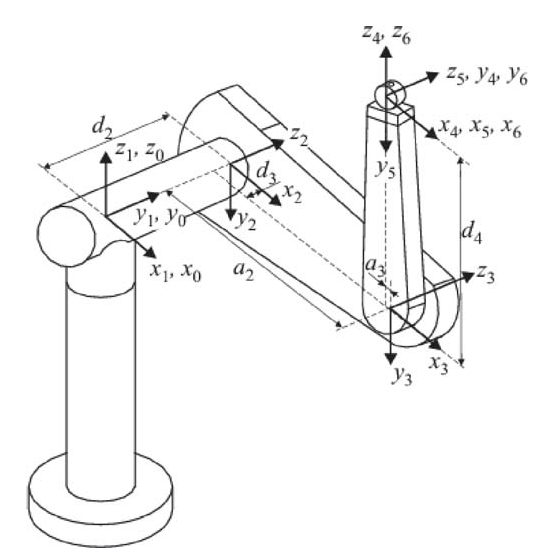
\includegraphics[width=0.5\linewidth]{pum}\caption{Schematic of a six degree of freedom PUMA robot} \label{pum}
\end{figure}
It is an industrial robotic arm developed by Victor Scheinman at pioneering robot company Unimation which was Initially developed for General Motors~\cite{rosheim1994robot,fu1987robotics}.\\
The robot has 6 degree of freedom with transformation for each of these degree of freedom having the form:
\begin{align}
A_i(\theta_i)=
\left [
\begin{array}{llrr}
\cos\theta_i & -\sin\theta_i & 0 & a_{i-1} \\
\sin\theta_i\cos\alpha_{i-1} & \cos\theta_i\cos\alpha_{i-1}  & -\sin\alpha_{i-1} & -d_i\sin\alpha_{i-1}\\
\sin\theta_i\sin\alpha_{i-1} & \cos\theta_i\sin\alpha_{i-1} & \cos\alpha_{i-1} & d_i\cos\alpha_{i-1}\\
0 & 0 & 0 & 1
\end{array} \right]\label{pumtrans}
\end{align}
where\\
$a_{i-1}$ is the perpendicular distance between the $(i-1)^{th}$ and the $i^{th}$ joint along the $x$-axis.\\
$\theta_i$ is the angle made by the $i^{th}$ linkage about the $z_i$-axis.\\
$\alpha_{i-1}$ is the angle between the $z_{i-1}$-axis and the $z_i$-axis.\\ 
and $d_i$ is the prismatic displacement of the $i^{th}$ linkage along $z_i$-axis.\\
The transformation in Eqn.~\ref{pumtrans} is gotten from the book, Robot manipulators: mathematics, programming, and control: the computer control of robot manipulators~\cite{paul1981robot}.\\
The transformation of each linkage is found using Eqn.~\ref{pumtrans}, giving the total transformation as:
\begin{equation}
    A(T)=A_2(\theta_2)A_3(\theta_3)A_4(\theta_4)A_5(\theta_5)A_6(\theta_6)
\end{equation}
By using Cliffore algebra, we can express $A(T)$ as
\begin{equation}
 A(T)=e^{-\left(\frac{\theta_2}{2}+\frac{\theta_3}{2}+\frac{\theta_4}{2}+\frac{\theta_5}{2}+\frac{\theta_6}{2}\right)e_2e_3}+e_1\sum_{i=1}^{6} a_i
\end{equation}
This transformation gives the total transformation covering all rotations and translations.\\
\section{Conclusion}
This results show that Clifford algebra and groups contains the symmetric tensor square of the adjoint representation of the group of rigid body motions $SE(3)$, as such, they can be used to represent transformation of bodies in the eucledean space in an algebraic  form. This representation makes analytic analysis and studies of motion of these kinds of object easy to view and analyze. The representation can also be used as the form used in algorithm used in computer programs.
\bibliographystyle{IEEEtran}
\bibliography{myrefs1}
\end{document}
